\documentclass{standalone}
\usepackage{graphicx}	
\usepackage{amssymb, amsmath}
\usepackage{color}

\usepackage{tikz}
\usetikzlibrary{intersections, backgrounds}

\definecolor{light}{RGB}{220, 188, 188}
\definecolor{mid}{RGB}{185, 124, 124}
\definecolor{dark}{RGB}{143, 39, 39}
\definecolor{highlight}{RGB}{180, 31, 180}
\definecolor{gray10}{gray}{0.1}
\definecolor{gray20}{gray}{0.2}
\definecolor{gray30}{gray}{0.3}
\definecolor{gray40}{gray}{0.4}
\definecolor{gray60}{gray}{0.6}
\definecolor{gray70}{gray}{0.7}
\definecolor{gray80}{gray}{0.8}
\definecolor{gray90}{gray}{0.9}
\definecolor{gray95}{gray}{0.95}

\newcommand*{\offset}{0.025}

\begin{document}

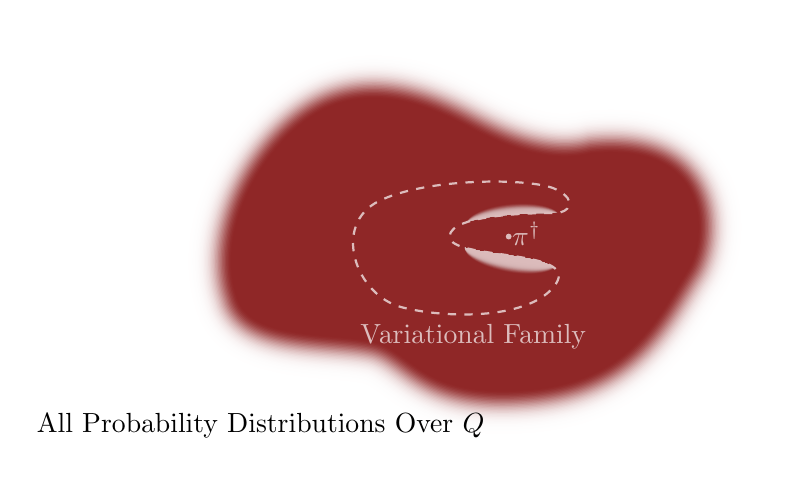
\begin{tikzpicture}[scale=0.15, thick]               

 \pgfmathsetmacro{\dx}{60}
 
 \foreach \i in {1, 0.975, ..., 0} {
   \pgfmathsetmacro{\prop}{100 * exp(-10.0 * \i * \i)};
   \colorlet{custom}{dark!\prop!white};
   \draw[line width={40 * \i}, color=custom] 
     (\dx + -20, -2)
    .. controls (\dx + -22, 4) and (\dx + -17, 12) .. (\dx + -12, 14)  
    .. controls (\dx + -7, 16) and (\dx + -2, 13) .. (\dx + 0, 12)
    .. controls (\dx + 2, 11) and (\dx + 6, 9) .. (\dx + 10, 10)
    .. controls (\dx + 20, 11) and (\dx + 20, 3) .. (\dx + 18, 0)
    .. controls (\dx + 15.5, -4) and (\dx + 13, -9.5) .. (\dx + 4, -10)
    .. controls (\dx + -4, -10.5) and (\dx + -5, -7) .. (\dx + -8, -6)
    .. controls (\dx + -11, -5) and (\dx + -19, -6) .. (\dx + -20, -2);
  }
  
  \fill [dark] (\dx + -20, -2)
    .. controls (\dx + -22, 4) and (\dx + -17, 12) .. (\dx + -12, 14)  
    .. controls (\dx + -7, 16) and (\dx + -2, 13) .. (\dx + 0, 12)
    .. controls (\dx + 2, 11) and (\dx + 6, 9) .. (\dx + 10, 10)
    .. controls (\dx + 20, 11) and (\dx + 20, 3) .. (\dx + 18, 0)
    .. controls (\dx + 15.5, -4) and (\dx + 13, -9.5) .. (\dx + 4, -10)
    .. controls (\dx + -4, -10.5) and (\dx + -5, -7) .. (\dx + -8, -6)
    .. controls (\dx + -11, -5) and (\dx + -19, -6) .. (\dx + -20, -2);
    
  \node [] at (\dx + -18, -13) { All Probability Distributions Over $Q$ };
  
  \begin{scope}
    \clip (\dx + 7, 7) 
      .. controls (\dx + 5, 8) and (\dx + -4, 8) .. (\dx + -8, 6) 
      .. controls (\dx + -12, 4) and (\dx + -10, -2) .. (\dx + -6, -3)
      .. controls (\dx + -2, -4) and (\dx + 5, -4) .. (\dx + 7, -1)
      .. controls (\dx + 9, 2) and (\dx + -2, 1) .. (\dx + -2, 3) 
      .. controls (\dx + -2, 5) and (\dx + 6, 5) .. (\dx + 7, 5)
      .. controls (\dx + 8, 5) and (\dx + 9, 6) .. cycle;
     
    \foreach \i in {0, 0.01,..., 1} {
      \fill[opacity={exp(-4 * \i * \i)}, light, rotate=5] (\dx + 3.5, -1.25) circle (4 and {1.5 * \i});      
    }
    \foreach \i in {0, 0.01,..., 1} {
      \fill[opacity={exp(-4 * \i * \i)}, light, rotate=-10] (\dx + 2, 12.4) circle (4 and {1.5 * \i});      
    }
  \end{scope}

  \draw[dashed, color=light] (\dx + 7, 7) 
    .. controls (\dx + 5, 8) and (\dx + -4, 8) .. (\dx + -8, 6) 
    .. controls (\dx + -12, 4) and (\dx + -10, -2) .. (\dx + -6, -3)
    .. controls (\dx + -2, -4) and (\dx + 5, -4) .. (\dx + 7, -1)
    .. controls (\dx + 9, 2) and (\dx + -2, 1) .. (\dx + -2, 3) 
    .. controls (\dx + -2, 5) and (\dx + 6, 5) .. (\dx + 7, 5)
    .. controls (\dx + 8, 5) and (\dx + 9, 6) .. cycle;
  
  \node[light] at (\dx + 0, -5.5) {Variational Family};
  
  \fill[light] (\dx + 3, 3) circle (7pt); 
  \node[light] at (\dx + 4.5, 3.25) {$\pi^{\dagger}$};  
  
\end{tikzpicture}

\end{document}   